\documentclass[11pt,a4paper]{article}
\usepackage[margin=2.2cm]{geometry}
\usepackage{amsmath}
\usepackage{graphicx}
\usepackage{float}
\usepackage{listings}

\lstset{basicstyle=\ttfamily\footnotesize, frame=single, numbers=left,
        numberstyle=\tiny, breaklines=true, columns=fullflexible}

\title{DEP512E -- HW1 Part A\\Newmark--$\beta$ Analysis of a SDOF System}
\author{Mesut ADALI - 801262107}
\date{19.10.2026}

\begin{document}
\maketitle

\section{Method}
The equation of motion is
\[
m\ddot{x} + c\dot{x} + kx = p(t), \qquad p(t) = -m\ddot{x}_g(t) \ \text{for ground motion.}
\]
The Newmark--$\beta$ method (incremental form) is used with $\beta = 1/4$ and $\gamma = 1/2$.
At each time step:
\[
\hat{k} = k + \frac{\gamma}{\beta\Delta t}c + \frac{m}{\beta\Delta t^2}, \qquad
\Delta\hat{p}_i = \Delta p_i + A\,\dot{x}_i + B\,\ddot{x}_i, \qquad
\Delta x_i = \frac{\Delta\hat{p}_i}{\hat{k}}
\]
\[
A = \frac{m}{\beta\Delta t} + \frac{\gamma}{\beta}c, \qquad
B = \frac{m}{2\beta} + \Delta t\left(\frac{\gamma}{2\beta}-1\right)c
\]
$\Delta\dot{x}_i$ and $\Delta\ddot{x}_i$ follow from $\Delta x_i$, and
$x_{i+1} = x_i + \Delta x_i$ (similarly for $\dot{x}$ and $\ddot{x}$).

\section{Code}
\begin{itemize}
  \item \texttt{newmark(m,c,k,p,dt,beta,gamma,x0,v0)}: applies the steps above and returns the
        displacement, velocity and acceleration vectors.
  \item Main part: defines the system and the loads, calls \texttt{newmark} and plots the results.
        The spring force is $f_S = kx$ and the damper force is $f_D = c\dot{x}$.
  \item System: $m = 1$ kg, $\omega_n = 2\pi$ rad/s, $\xi = 0.05$, so
        $k = m\omega_n^2 = 39.48$ N/m and $c = 2\xi m\omega_n = 0.628$ N\,s/m.
  \item Problem 1: $p(t) = 2\sin(\pi t/2)$, $\Delta t = 0.01$ s, 20 s.
  \item Problem 2: ground acceleration from \texttt{ground\_acc.txt}, $\Delta t = 0.005$ s
        (7860 points, 39.3 s), $p = -m\ddot{x}_g$.
\end{itemize}

\section{Results -- Problem 1}
\begin{figure}[H]
\centering
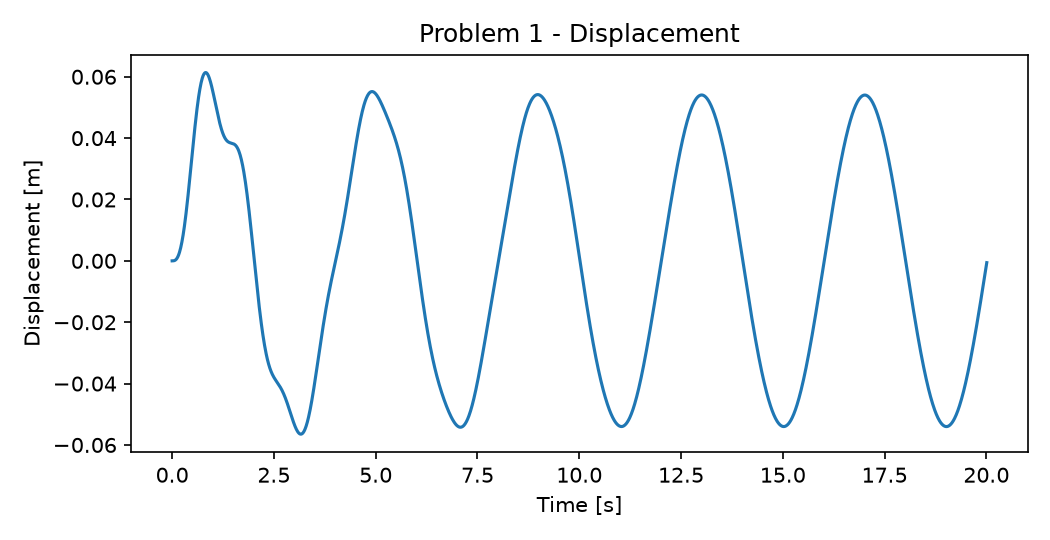
\includegraphics[width=0.49\textwidth]{figures/Problem_1_Displacement.png}
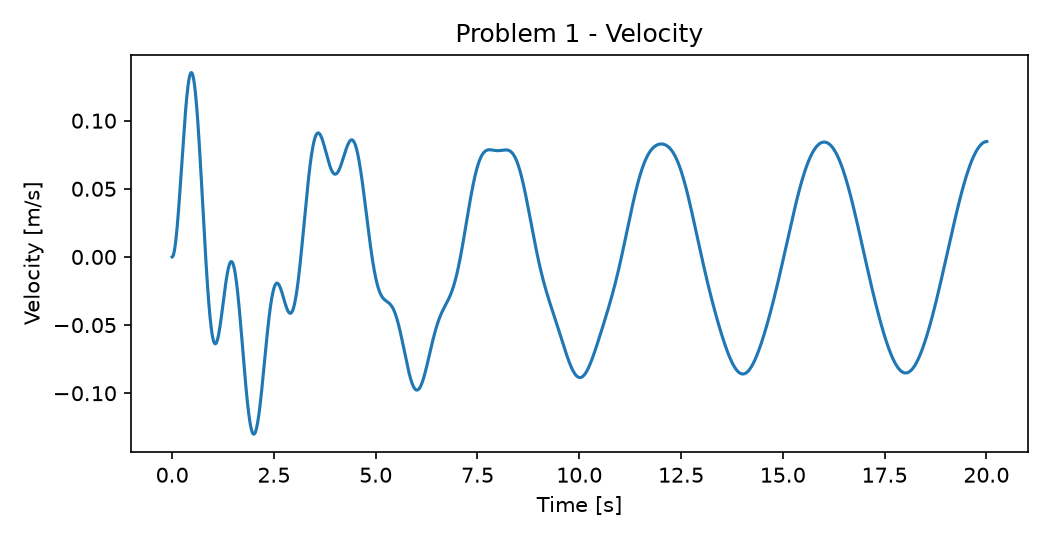
\includegraphics[width=0.49\textwidth]{figures/Problem_1_Velocity.png}
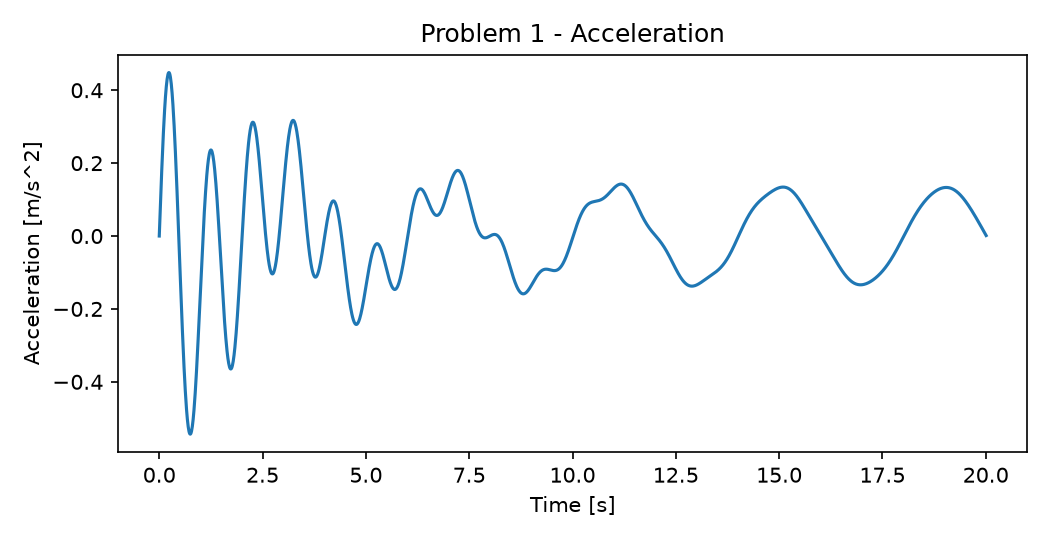
\includegraphics[width=0.49\textwidth]{figures/Problem_1_Acceleration.png}
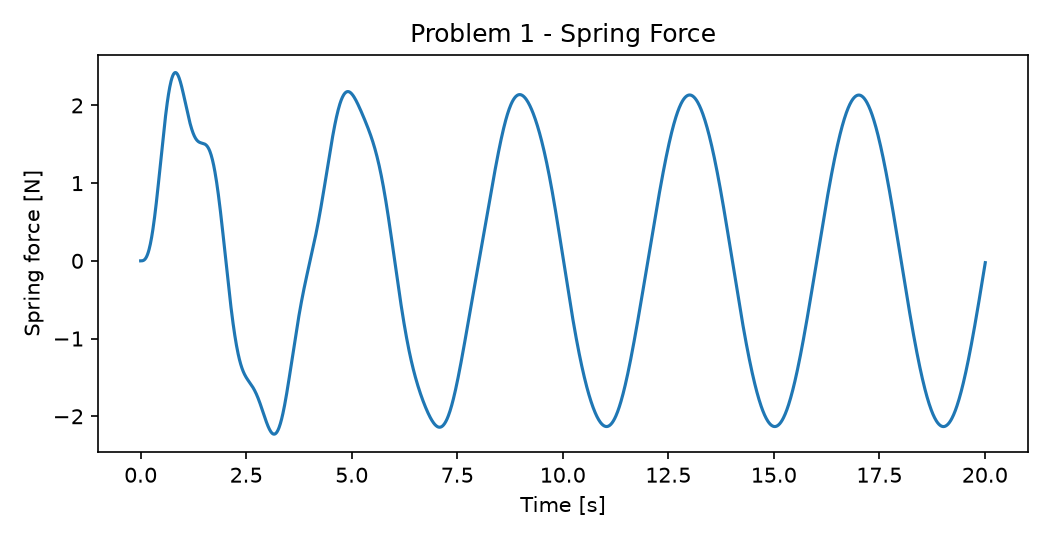
\includegraphics[width=0.49\textwidth]{figures/Problem_1_Spring_Force.png}
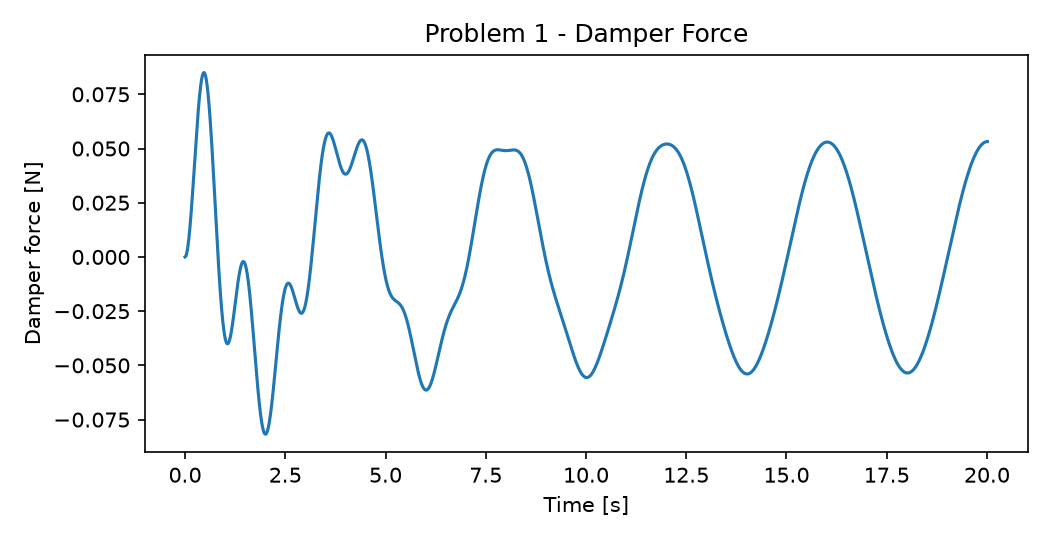
\includegraphics[width=0.49\textwidth]{figures/Problem_1_Damper_Force.png}
\caption{Problem 1: time histories.}
\end{figure}

\begin{figure}[H]
\centering
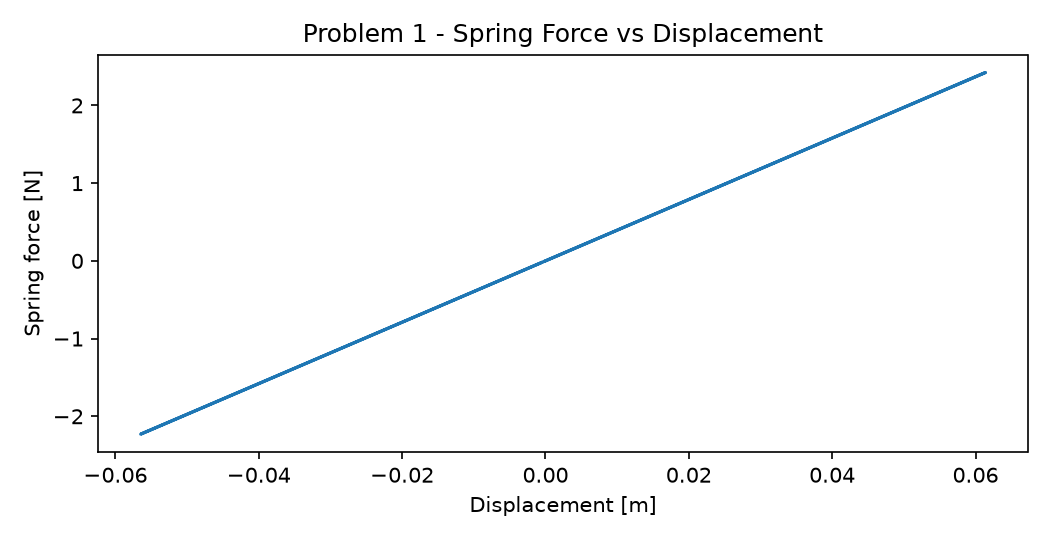
\includegraphics[width=0.49\textwidth]{figures/Problem_1_Spring_Force_vs_Displacement.png}
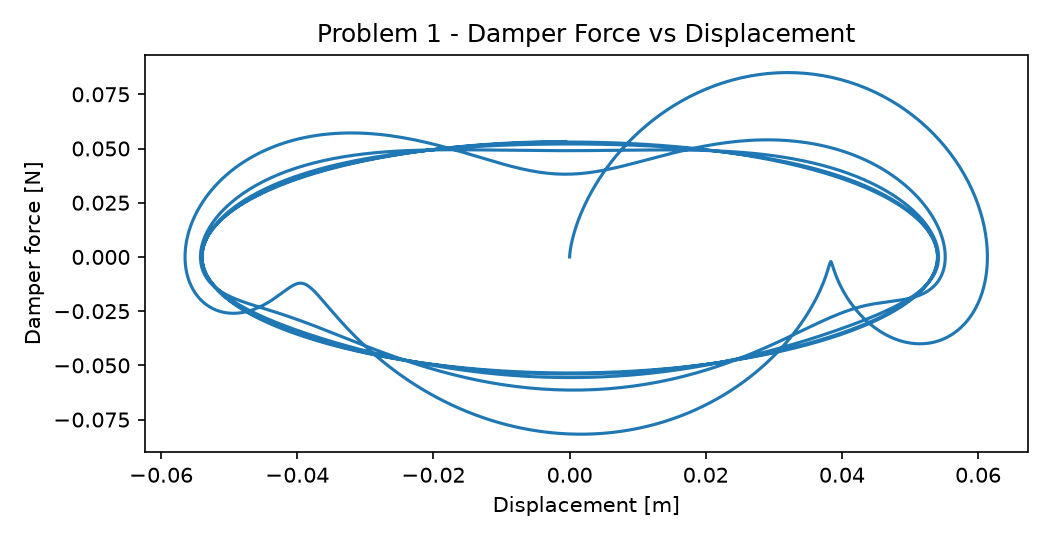
\includegraphics[width=0.49\textwidth]{figures/Problem_1_Damper_Force_vs_Displacement.png}
\caption{Problem 1: displacement vs spring force and damper force.}
\end{figure}

\section{Results -- Problem 2}
\begin{figure}[H]
\centering
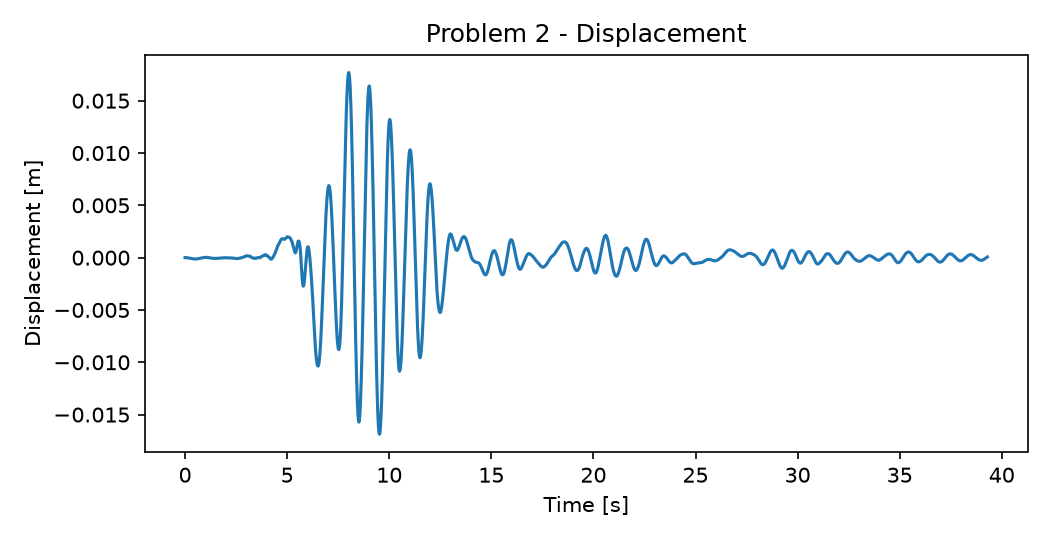
\includegraphics[width=0.49\textwidth]{figures/Problem_2_Displacement.png}
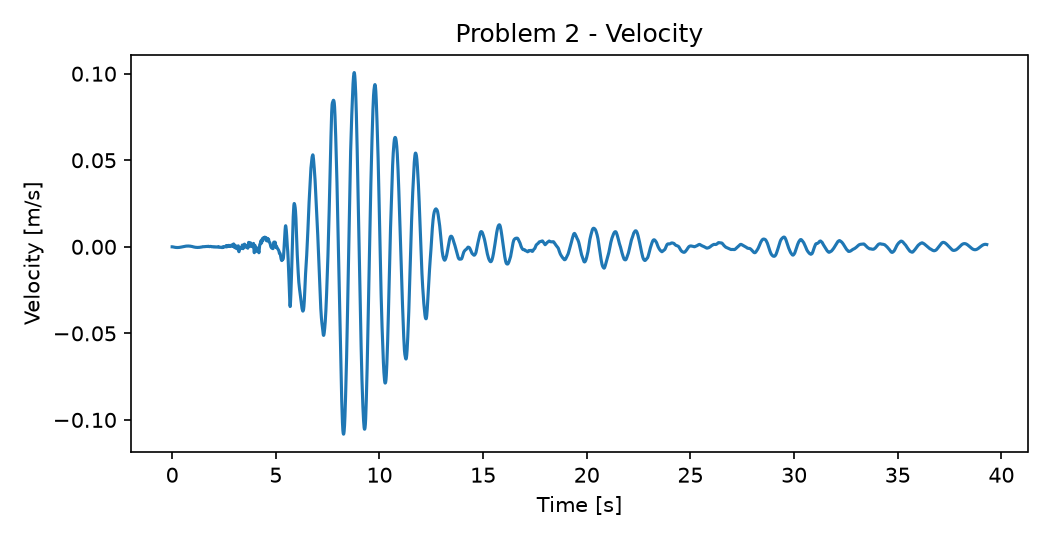
\includegraphics[width=0.49\textwidth]{figures/Problem_2_Velocity.png}
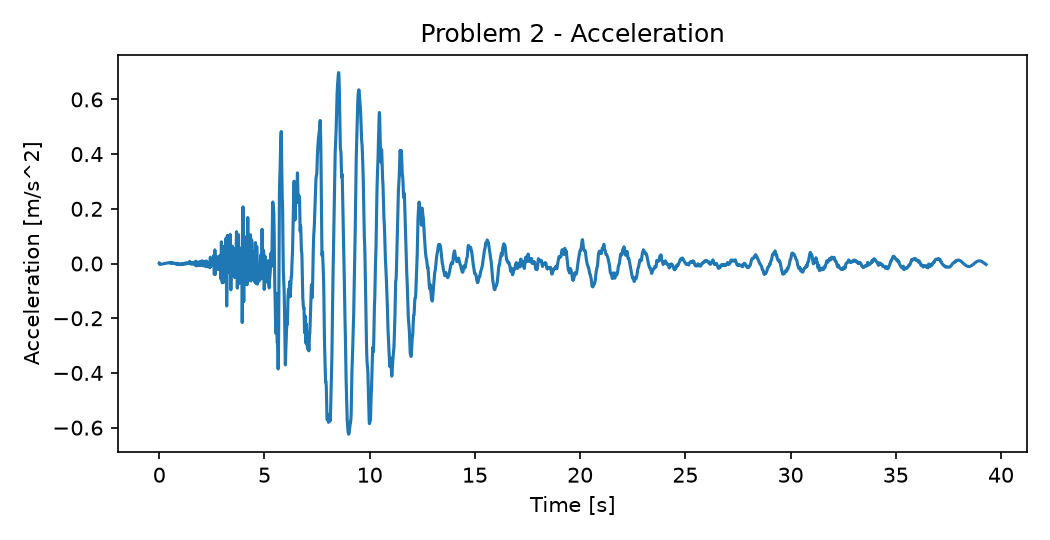
\includegraphics[width=0.49\textwidth]{figures/Problem_2_Acceleration.png}
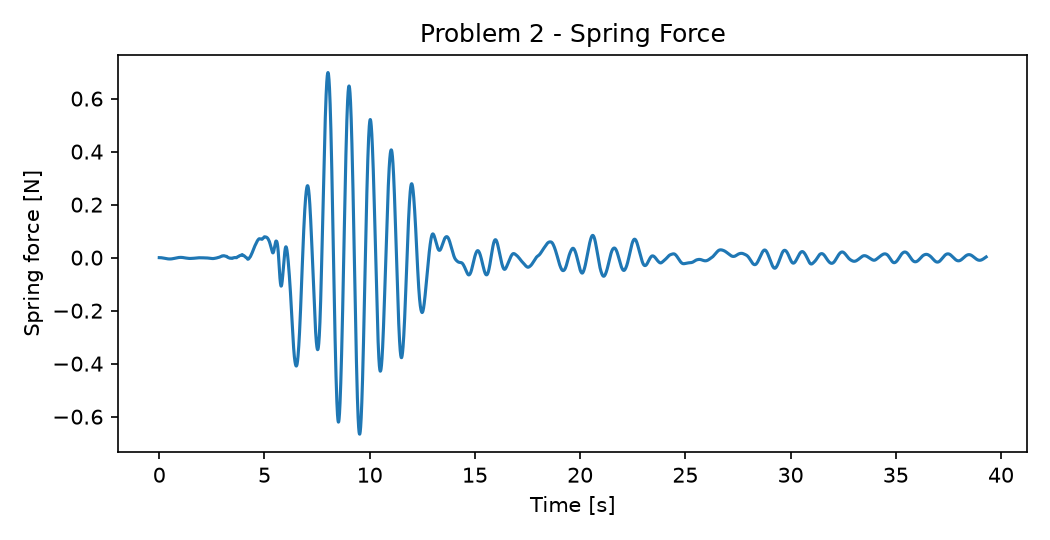
\includegraphics[width=0.49\textwidth]{figures/Problem_2_Spring_Force.png}
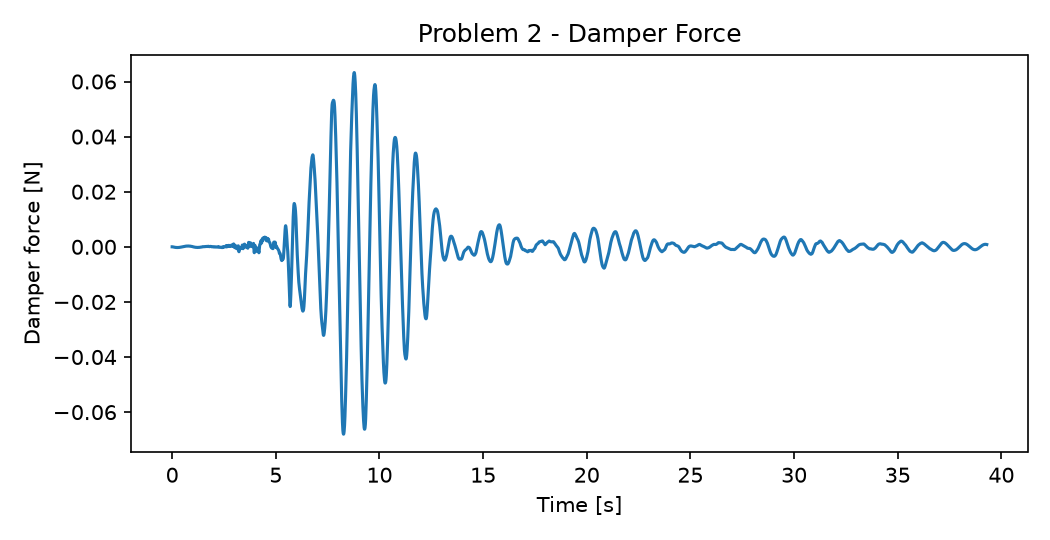
\includegraphics[width=0.49\textwidth]{figures/Problem_2_Damper_Force.png}
\caption{Problem 2: time histories.}
\end{figure}

\begin{figure}[H]
\centering
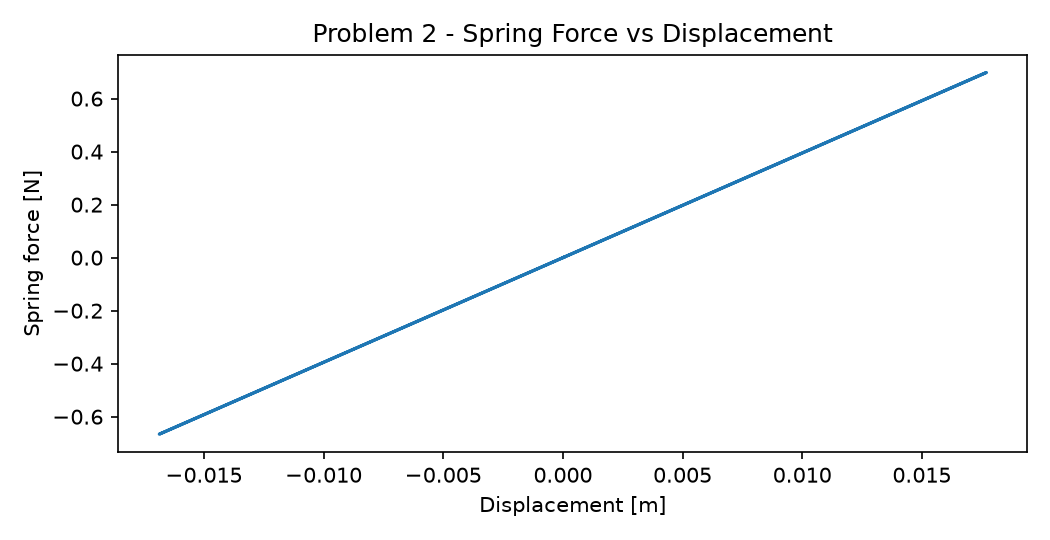
\includegraphics[width=0.49\textwidth]{figures/Problem_2_Spring_Force_vs_Displacement.png}
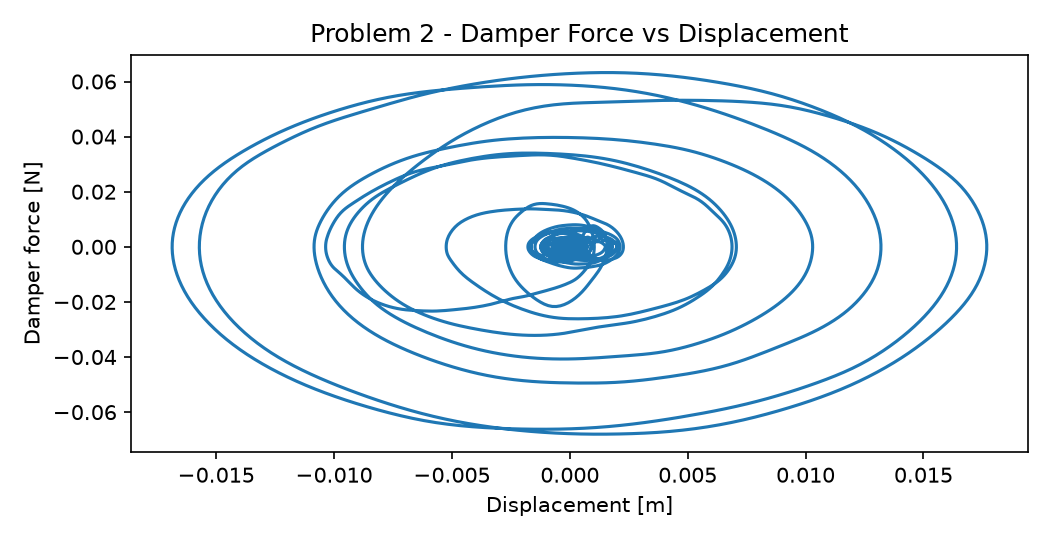
\includegraphics[width=0.49\textwidth]{figures/Problem_2_Damper_Force_vs_Displacement.png}
\caption{Problem 2: displacement vs spring force and damper force.}
\end{figure}

\appendix
\section{Python Code}
\lstinputlisting[language=Python]{"DEP512E-HW1-Part A.py"}

\end{document}
